%! TEX program = pdflatex

\documentclass[oneside,solution]{tmpl}

\usepackage[utf8]{inputenc}
\usepackage[english,ukrainian]{babel}

\title{Домашня робота}
\author{Захаров Дмитро}
\studentID{МП-31}
\instructor{Ігнатович С.Ю.}
\date{\today}
\duedate{23:59 22 квітня, 2024}
\assignno{6}
\semester{Весняний семестр 2024}
\mainproblem{Граничні цикли}

\begin{document}

\maketitle

% \startsolution[print]

\problem{Напівстійкий цикл.}

\textbf{Умова.} Розглянемо систему
\begin{equation}
    \begin{cases}
        \dot{r} = r(1-r)^2 \\
        \dot{\varphi} = 1
    \end{cases}
\end{equation}

Вона теж має граничний цикл, що є колом радіуса $1$. Але, на відміну від системи 2, цей граничний цикл є напівстійким: частина фазових траєкторій наближається до нього, а частина -- віддаляється. Доведіть цей факт, тобто з'ясуйте, які траєкторії наближаються, а які віддаляються. Нарисуйте фазовий портрет цієї системи.

\textbf{Розв'язок.} Оскільки рівняння $\dot{\varphi}=1$ лише задає умову на те, що траєкторія ``обертається'' з постійною кутовою швидкістю, то сконцетруємось на рівнянні $\dot{r} = r(1-r)^2$. Вигляд траєкторії головним чином залежить від початкової умови $r(0) := r_0$. Оскільки $r>0$, бо ми знаходимось у полярних координатах (випадок $r=0$ буде просто відповідати знаходженні у початку координат), то тут принципово маємо три випадки:
\begin{itemize}
    \item $r_0=1$: згідно рівнянню, $\dot{r} \equiv 0$, а тому радіус-вектор буде залишатись з постійною довжиною $1$ і обертатись з постійною кутовою швидкістю. Отже, маємо рівномірний рух по колу.
    \item $r_0 \in (0,1)$: маємо, що початкова швидкість $\dot{r}(0) > 0$, тобто радіус-вектор почне збільшуватись. Помітимо, що при цьому, коли радіус-вектор буде близьким до $1$, то швидкість буде постійно зменьшуватись і в решті-решт наближатись до $0$. Тобто, траєкторія асимптотично вийде на те саме коло у випадку $r_0=1$.
    \item $r_0>1$: початкова швидкість $\dot{r}(0)$ знову буде додатною (це обумовлено тим, що доданок $(1-r)^2$ піднесений у парний степінь), причому чим далі $r$ від $1$, тим більше це значення. Отже, траєкторія буде віддалятись на нескінченність.
\end{itemize}

Отже, будь-які траєкторії, що починаються всередині кола $r=1$ (окрім нестабільної точки $r=0$) будуть виходити на це коло, а ось все, що залишилось за ним, буде нескінченно віддалятись. Отже, дійсно маємо напівстійкість. Це можна побачити на Рисунку \ref{fig:problem_1}.

\begin{figure}
    \centering
    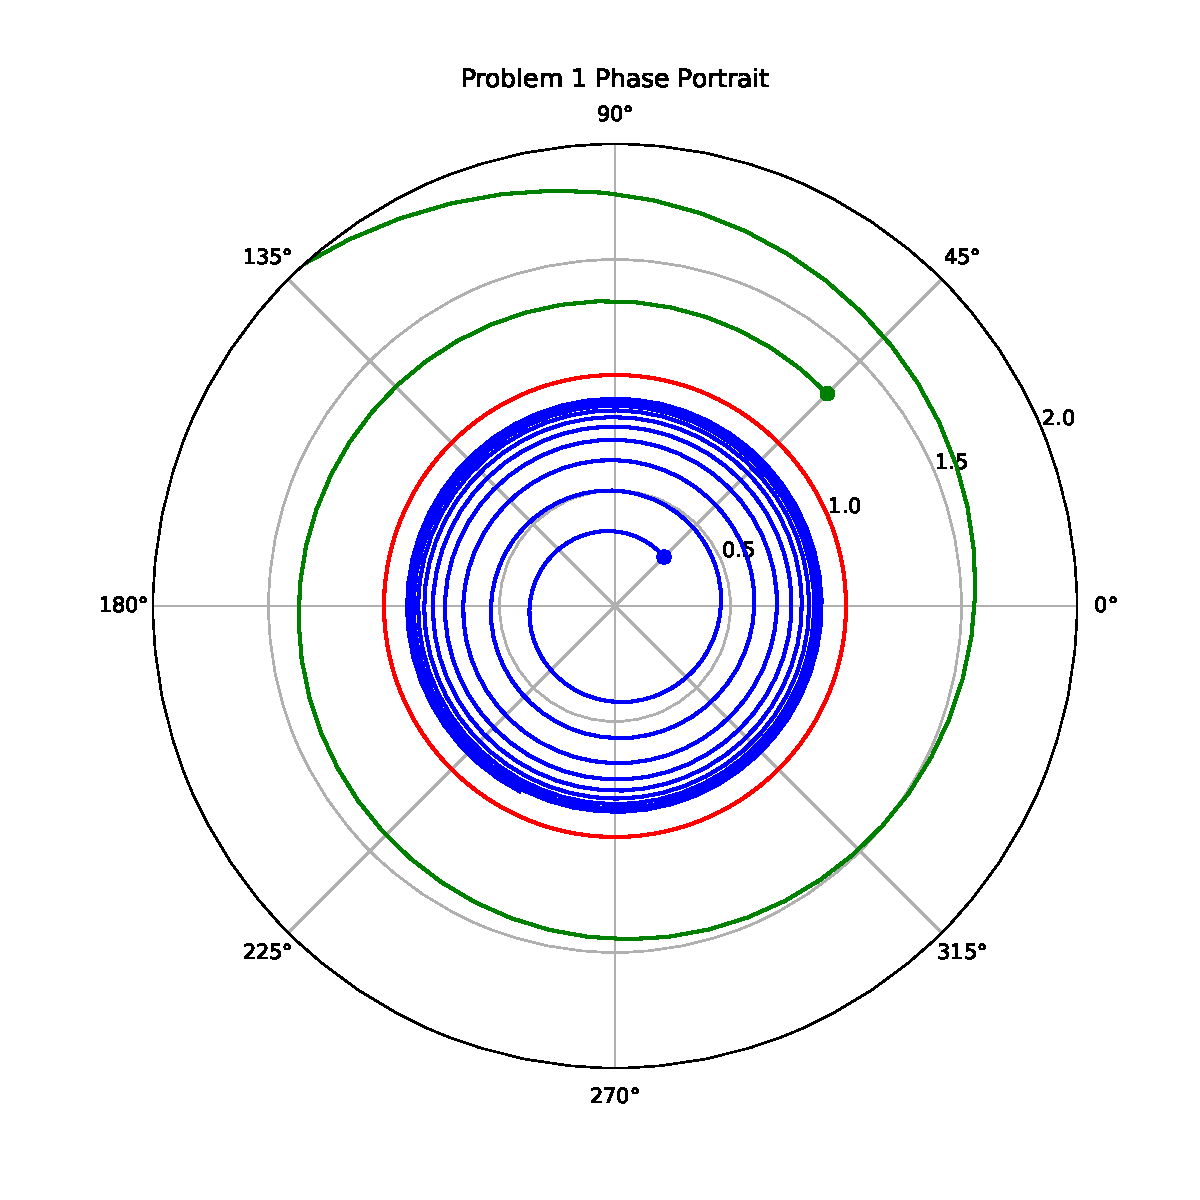
\includegraphics[width=0.7\textwidth]{images/hw_6/problem_1.pdf}
    \caption{Фазовий портрет для системи з задачі $1$. \textcolor{blue}{Синім} показано траєкторію для точки, що починає рух всередині круга $r=1$, а \textcolor{green}{зеленим} -- за кругом.}
    \label{fig:problem_1}
\end{figure}


\problem{Кількість граничних циклів.}

\textbf{Умова.} Розглянемо систему
\begin{equation}
    \begin{cases}
        \dot{r} = r(1-r)(r-2) \\
        \dot{\varphi} = 1
    \end{cases}
\end{equation}

Скільки граничних циклів має ця система? Які вони з точки зору стійкості?

\textbf{Розв'язок.} Знову концентруємось на рівнянні $\dot{r}=r(1-r)(r-2)$. Його нулі праворуч -- це $r=0,r=1,r=2$. Рівняння $r=0$ задає точку спокою, що знаходиться у початку координат. У свою чергу, $r=1$ та $r=2$ задають два кола радіуса $1$ та $2$, відповідно. Далі, розглядаємо наступні проміжки для початково значення $r(0):=r_0$:
\begin{itemize}
    \item $r_0 \in (0,1)$: в цьому випадку початкова швидкість від'ємна, а отже точка почне наближуватись до $0$. Ближче до $0$, швидкість зміни довжини радіус-вектора буде наближатись до $0$, а отже асимптотично траєкторія буде ``тормозити'' у початок координат.
    \item $r_0 \in (1,2)$: тут початкова швидкість буде додатньою, а отже точка буде віддалятись від кола $r=1$. Далі, швидкість буде тормозити, поки точка не вийде на коло $r=2$.
    \item $r_0>2$: початкова швидкість від'ємна і при наближенні до $r=2$ буде тормозити. Таким чином, знову траєкторія буде виходити на коло $r=2$.
\end{itemize}

Таким чином, маємо два граничні цикли: $r=1$ -- нестійкий цикл, а також $r=2$ -- стійкий.

\problem{Система з трьома різними циклами.}

\textbf{Умова.} Придумайте систему, у якої три граничні цикли: один стійкий, один напівстійкий і один нестійкий. Випишіть систему і нарисуйте її фазовий портрет.

\textbf{Розв'язок.} В якості такої системи візьмемо систему з завдання 2, але додамо доданок $(r-3)^2$ до системи:
\begin{equation}
    \begin{cases}
        \dot{r} = \alpha r(1-r)(r-2)(r-3)^2 \\
        \dot{\varphi} = 1
    \end{cases}, \; \alpha > 0
\end{equation}

Що це нам дає? По-перше, $r=1$ та $r=2$ все ще будуть нестійким та стійким циклом, відповідно, оскільки доданок $(r-3)^2$ не впливатиме на знаки похідних. Отже, якщо $r_0 \in (2,3)$, то точка буде все ще виходити на коло $r=2$. В свою чергу, якщо $r_0 > 3$, то точка буде рухатись в тому самому напрямку, що і при $r_0 \in (2,3)$, але вже гранично ``накручуватись'' на граничний цикл $r=3$. Таким чином, як і в завданні 1, він буде напівстійким. Фазовий портрет зображений на Рисунку \ref{fig:problem_3}. 

\begin{figure}
    \centering
    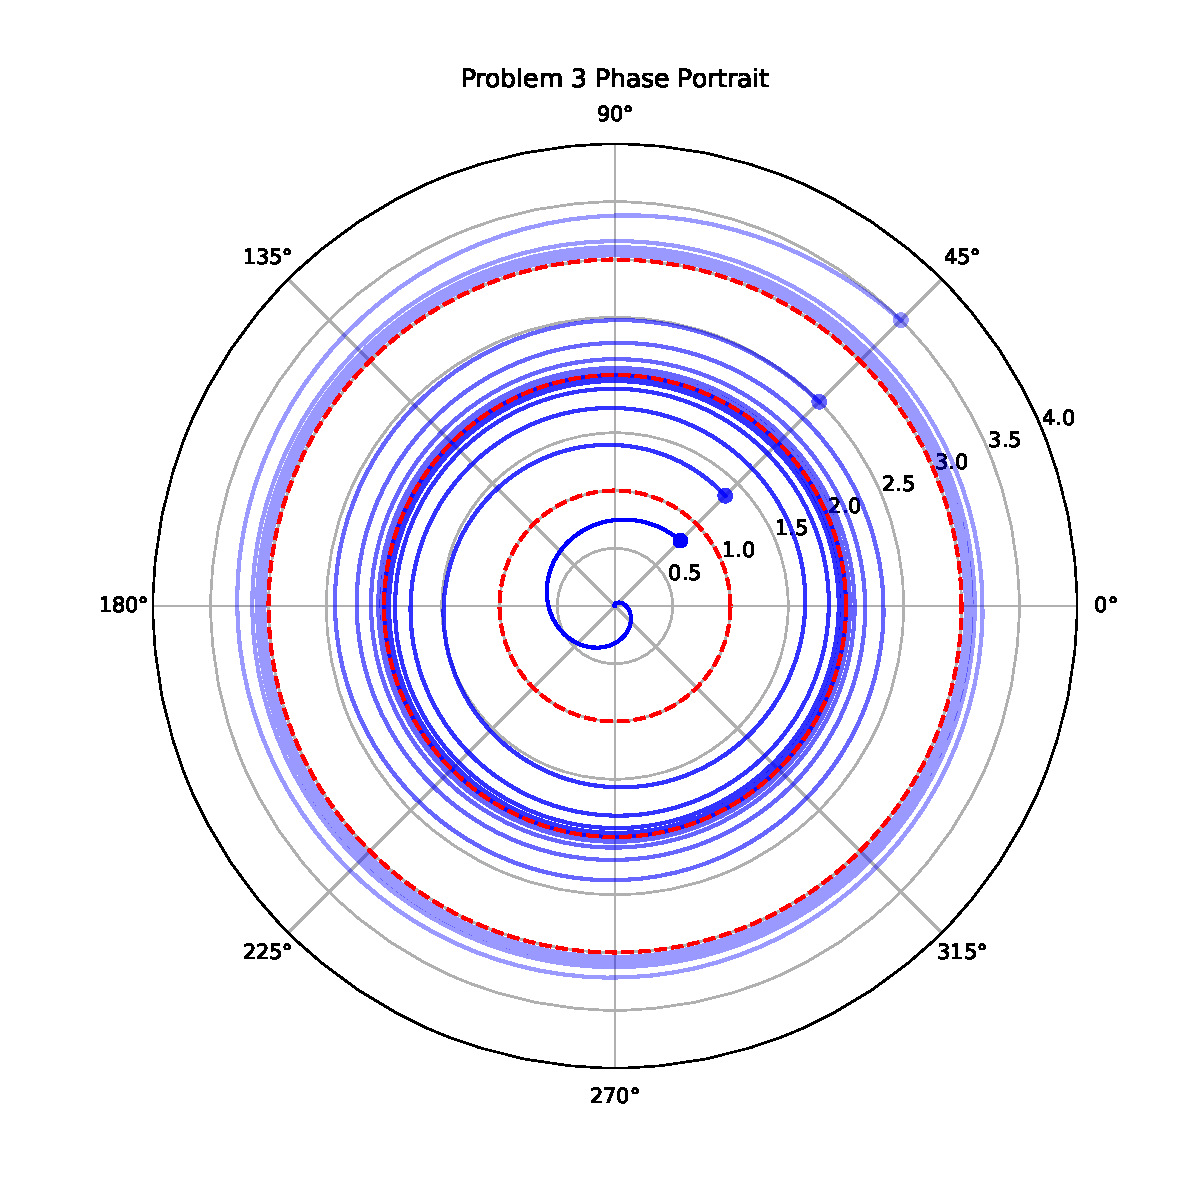
\includegraphics[width=0.7\textwidth]{images/hw_6/problem_3.pdf}
    \caption{Фазовий портрет для системи з задачі $3$ для $\alpha=\frac{1}{15}$. Різними відтінками \textcolor{blue}{синього} відмічено різні траєкторії в залежності від початкової довжини радіус-вектора. \textcolor{red}{Червоним} пунктиром відмічено три граничні цикли: $r=1,r=2,r=3$. Бачимо, що на коло $r=1$ не намотується жодна траєкторія, на $r=2$ -- дві траєкторії з обох боків, а на $r=3$ -- тільки одна ззовні кола $r=3$.}
    \label{fig:problem_3}
\end{figure}

\end{document}
